
%(BEGIN_QUESTION)
% Copyright 2014, Tony R. Kuphaldt, released under the Creative Commons Attribution License (v 1.0)
% This means you may do almost anything with this work of mine, so long as you give me proper credit

Calculate the necessary size of the capacitor to give this circuit a total impedance ($Z_{total}$) of 4 k$\Omega$, at a power supply frequency of 100 Hz:

$$\includegraphics[width=15.5cm]{i01035x01.eps}$$

Also calculate the following phase shift angles ($\theta$) between voltage and current for each component in this series circuit:

\vskip 20pt

Phase shift between resistor voltage drop and resistor current = \underbar{\hskip 50pt} degrees

\vskip 20pt

Phase shift between capacitor voltage drop and capacitor current = \underbar{\hskip 50pt} degrees

\vskip 20pt

Phase shift between source voltage and source current = \underbar{\hskip 50pt} degrees

\vfil

\underbar{file i01035}
\eject
%(END_QUESTION)





%(BEGIN_ANSWER)

This is a graded question -- no answers or hints given!

%(END_ANSWER)





%(BEGIN_NOTES)

The given resistance value of 2200 ohms forms the adjacent side of a right triangle, where the capacitive reactance ($X_C$) forms the opposite side and the total series impedance ($Z$) forms the hypotenuse.  If the hypotenuse has a length of 4 k$\Omega$ and the adjacent has a length of 2.2 k$\Omega$, then the opposite must be equal to:

$$X = \sqrt{Z^2 - R^2}$$

$$X = \sqrt{4000^2 - 2200^2}$$

$$X = 3340.66$$

\vskip 10pt

At this point we can work the capacitive reactance formula backwards to solve for the necessary value of $C$ to give us this much reactance at a circuit frequency of 100 Hz:

$$X_C = {1 \over {2 \pi f C}}$$

$$C = {1 \over {2 \pi f X_C}}$$

$$C = {1 \over {2 \pi (100) (3340.66)}}$$

$$C = 0.476 \> \mu \hbox{F}$$

\vskip 10pt

Phase shifts for resistors and capacitors are defined by those components' natures: 0$^{o}$ for resistors and $-$90$^{o}$ for capacitors:

\vskip 10pt

Phase shift between resistor voltage drop and resistor current = \underbar{\bf 0 degrees}

\vskip 10pt

Phase shift between capacitor voltage drop and capacitor current = \underbar{\bf 90 degrees, voltage lagging}

\vskip 10pt

Phase shift between voltage and current for the source may be calculated from the given total impedance and resistance of the circuit, since a similar triangle relates total source voltage to circuit current (that current having the same phase as resistor voltage).  Calculating $\theta$ for a right triangle with a hypotenuse of 4000 and an adjacent of 2200 yields 28.8$^{o}$:

\vskip 10pt

Phase shift between source voltage and source current = \underbar{\bf 28.8 degrees, voltage lagging}


%INDEX% Electronics review: AC reactance and impedance

%(END_NOTES)


